\section*{Paper Title}
\textbf{\textit{Order Space-Based Morphology for Color Image Processing.}}


\subsubsection*{Abstract}
Mathematical morphology in image processing is a fundamental tool based on order statistics, while binary and grayscale images, whose pixels can be sorted by their pixel values, i.e., each pixel can be labeled in a specific order. However, considering a three channel RGB image, each pixel has three numbers corresponding to three color channels; therefore, it is difficult to sort color pixels uniquely. This paper proposed a method for unifying the orders of pixels sorted in each color channel separately, where we consider that a pixel exists in a three-dimensional space called order space, and derive a single order by a monotonically non-decreasing function defined on the order space. The proposed method treats three orders of pixels sorted in respective color channels equally; hence, it is consistent with the original morphological operations for gray-scale images that we have learned in class.

\section*{Motivation}
For the first-half of the semester, we focus on image processing for single-channel(gray-scale) images only, and for RGB images, we tend to split them into 3 individual channel and process them respectively. However, despite it make sense to handle each channel individually, we are curious that whether it is possible to have a end-to-end method to process RGB images. Hence we want to extend morphological processing from gray-scale images to RGB images.
%\newpage

\section*{Problem Definition}
Given $n$ pixels $f_1$, $f_2$, ..., $f_n$, each with $R$, $G$, $B$ values. Find the order $O_1$, $O_2$, ..., $O_n$ of the pixels, where $O_i$ is the order of $f_i$ among all pixels.


% \newpage

\section*{Introduction}
% Mathematical morphology is a theory that originated in the 1960s for treating the shape of objects in images based on set theory and lattice theory. Mathematical morphology has a wide range of applications in digital image processing, where the development of basic techniques for binary and gray-scale images is almost complete. However, mathematical morphology for color images and higher-dimensional images is still under study because of the difficulty and uncertainty of ordering vector data, such as color vectors or pixels, in color images.\\

Mathematical morphology is a large for in the realm of digital image processing that focuses on the analysis and processing of geometric structures within images. It has a wide range of applications including noise reduction, shape analysis, image enhancement, etc., where the development of basic techniques for binary and gray-scale images is almost complete. However, mathematical morphology for color images and higher-dimensional images is still under study because of the difficulty and uncertainty of the orderings, such as color pixels in color images, having more than one channel that needed to be sorted.\\

This paper introduced the concept of the order space for color images, which is a three-dimensional space where axes are the orders of pixels in three color channels: \textbf{R}, \textbf{G}, and \textbf{B}. We first sort the pixels in each channel separately, then as a result, we obtain a triplet of orders for each pixel $(o_{\xi}^{R}, o_{\xi}^{G}, o_{\xi}^{B})$, which we can place it as a point in the proposed order space. Lastly, we compute a single order from the triplet of orders from 3D to 1D using some selected functions, and then apply morphological operations based on the computed single order of pixels.
% \newpage

\section*{Algorithm}
\begin{algorithm}[H]
\caption{Mapping from RGB color space to order space}
\KwData{a set of pixels $\{f_{i+k,j+l} = [f_{i+k,j+l}^{R}, f_{i+k,j+l}^{G}, f_{i+k,j+l}^{B}]\ |\ (k,l) \in S\}$ (S is the structuring element used in operation)}
\KwResult{a set of coordinates in order space $\{(o_{\xi}^{R}, o_{\xi}^{G}, o_{\xi}^{B})\ | \ \xi \in \{1,2,\ldots, |S|\}\}$}

Assign serial numbers $\xi \in \{1,2,\ldots, |S|\}$ to all pixels in the required set to have a set of re-indexed pixels  $\{f_{\xi} = [f_{\xi}^{R}, f_{\xi}^{G}, f_{\xi}^{B}]\ |\ \xi \in \{1,2,\ldots, |S|\}$.

\For{$X \in \{R, G, B\}$}{
    $[a_{1}^{X}, a_{2}^{X}, \ldots, a_{|S|}^{X}] = argsort(f_{1}^{X}, f_{2}^{X}, \ldots, f_{|S|}^{X})$;
    
    \For{$\xi \in \{1,2,\ldots, |S|\}$}{
        $o_{a_{\xi}^{X}}^{X} = \xi$;
    }
}
\Return $\{(o_{\xi}^{R}, o_{\xi}^{G}, o_{\xi}^{B})\ | \ \xi \in \{1,2,\ldots, |S|\}\}$
\end{algorithm}

% Order Space-Based Morphology for Color Image Processing in the paper
\section*{Order Space-Based Morphology for Color Image Processing}

Let $F = [f_{ ij }] $ be an RGB color image, where $f_{ ij } = [f_{ ij }^{R}, f_{ ij }^{G}, f_{ ij }^{B}] $ denotes the RGB color vector at the position $(i,j)$ in F. \\

We sort the color components covered by a structuring element in ascending order of their values, e.g., 
$f^{R}_{i+k(a_{1}^{R}),\ j+l(a_{1}^{R})  } \leq 
f^{R}_{i+k(a_{2}^{R}),\ j+l(a_{2}^{R})  } \leq \ldots \leq
f^{R}_{i+k(a_{5}^{R}),\ j+l(a_{5}^{R})  }$
for the R component with a structuring element S with five pixels, where $a_{ 1 }^{R},a_{ 2 }^{R},\ldots,a_{ 5 }^{R}$
 denote the sorted indices of pixels covered by S. $k(a_{i}^{R})$
 and $l(a_{i}^{R})$
 denote the vertical and horizontal relative coordinates of the pixel corresponding to $a_{i}^{R}$, respectively.\\

 Let $\xi=a_{\eta}^{R} (for\ \eta=1,2,\ldots,5)$
 be a function where a pixel index $\xi$ is related to an order $\eta$
 given by the above sorting process. 
 Then, we consider the inverse function of $\xi=a_{\eta}^{R}$
 as $\eta=o_{\xi}^{R} = (a^{R})_{\xi}^{-1}$. Similarly, we can sort the G component and B component, considering the inverse function to get $o_{\xi}^{G}$ and $o_{\xi}^{B}$.\\
 
 In the 3D order space, an RGB color pixel with an index $\xi$
 is represented by a triplet $(o_{\xi}^{R}, o_{\xi}^{G}, o_{\xi}^{B})$
. To define dilation and erosion for an RGB color image, we need to reduce the triplet $(o_{\xi}^{R}, o_{\xi}^{G}, o_{\xi}^{B})$ to a singlet $o_{\xi}$.There are some equations to achieve this:
\begin{center}
$o_{\xi}^{S}=o_{\xi}^{R}+o_{\xi}^{G}+o_{\xi}^{B}$\\
\
\\
$o_{\xi}^{P}=o_{\xi}^{R}o_{\xi}^{G}o_{\xi}^{B}$\\
\
\\
$o_{\xi}^{M}=median(o_{\xi}^{R},o_{\xi}^{G},o_{\xi}^{B})$
\\
\end{center}
Once we reduce $(o_{\xi}^{R}, o_{\xi}^{G}, o_{\xi}^{B})$ to $o_{\xi}$, we can define the dilation and erosion of F by S as follows:
\begin{center}
$D(F,S) = [d_{ij}], \  d_{ij}=f_{\xi^{max}}\ \ \xi^{max}=arg \mathop{max\ \ o_{\xi}}\limits_{\xi\in\{1,2,\ldots,|S|\}} $
\\
\ 
\\
$E(F,S) = [e_{ij}], \  e_{ij}=f_{\xi^{min}}\ \ \xi^{min}=arg \mathop{min\ \ o_{\xi}}\limits_{\xi\in\{1,2,\ldots,|S|\}} $
\end{center}
Also, we can combine the above dilation and erosion operations for defining opening and closing operations as follows:
\begin{center}
$O(F,S)=D(E(F,S),S)$
\\
\ 
\\
$C(F,S)=E(D(F,S),S)$
\end{center}
Combining the above opening and closing operations, we can define open–closing and close–opening operations as follows:
\begin{center}
$OC(F,S)=C(O(F,S),S)$
\\
\ 
\\
$CO(F,S)=O(C(F,S),S)$
\end{center}
% \newpage


% Fuzzy Morphological Operations by Exponentially Weighted Averaging in the paper
\section*{Fuzzy Morphological Operations by Exponentially\\ Weighted Averaging}

We introduce an exponentially weighted averaging method to make fuzzy order space-based morphological operations.\\

Assume that an order $o_{\xi}$
 for $\xi\in{1,2,\ldots,|S|}$
 is obtained from a set of triplets $(o_{\xi}^{R}, o_{\xi}^{G}, o_{\xi}^{B})$. Then, we define a fuzzy dilation with an exponentially weighted averaging method as follows:\\
\begin{center}
 $D^{FUZ}(F,S,\alpha) = [d_{ij}^{FUZ}], \  d_{ij}=\frac{\displaystyle\sum_{\xi=1}^{|S|} exp (\alpha o_{\xi})f_{\xi}}{\displaystyle\sum_{\xi=1}^{|S|} exp (\alpha o_{\xi})}$ , \\
 \end{center}
 
 where exp denotes the exponential function defined by $exp(x)=e^{x}$
, where e is a constant called Euler’s number and $\alpha$
 is a positive constant for controlling the fuzziness.\\

 Similarly, we can define a fuzzy erosion as follows:
 \begin{center}
 $E^{FUZ}(F,S,\alpha) = [e_{ij}^{FUZ}], \  e_{ij}=\frac{\displaystyle\sum_{\xi=1}^{|S|} exp (-\alpha o_{\xi})f_{\xi}}{\displaystyle\sum_{\xi=1}^{|S|} exp (-\alpha o_{\xi})}$ , \\
 \end{center}
Combining these operations, we can define fuzzy opening and closing operations as follows:
\begin{center}
$O^{FUZ}(F,S,\alpha)=D^{FUZ}(E^{FUZ}(F,S,\alpha),S,\alpha)$
\\
\ 
\\
$C^{FUZ}(F,S,\alpha)=E^{FUZ}(D^{FUZ}(F,S,\alpha),S,\alpha)$
\end{center}
From these, we further define fuzzy open–closing and close–opening operations as follows:
\begin{center}
$OC^{FUZ}(F,S,\alpha)=C^{FUZ}(O^{FUZ}(F,S,\alpha),S,\alpha)$
\\
\ 
\\
$CO^{FUZ}(F,S,\alpha)=O^{FUZ}(C^{FUZ}(F,S,\alpha),S,\alpha)$
\end{center}

% \newpage

\section*{Expected Experimental Result}

\textbf{Figure 1} is a noisy input image including $10\% $ impulse noise, where $6553$ out of $256×256=65,536$ pixels are corrupted with impulse noise for evaulation compared with Wang’s hypergraph-based method (Wang, J.; Liang, G.; Wu, Y.; Li, Y.; Hu, J. New colour morphological operators on hypergraph. \textit{IET Image Process.} \textbf{2018}, 12, 690–695.)
\begin{figure}[H]
    \label{img:figure6}
    \centering
    \begin{subfigure}[t]{.4\textwidth}
    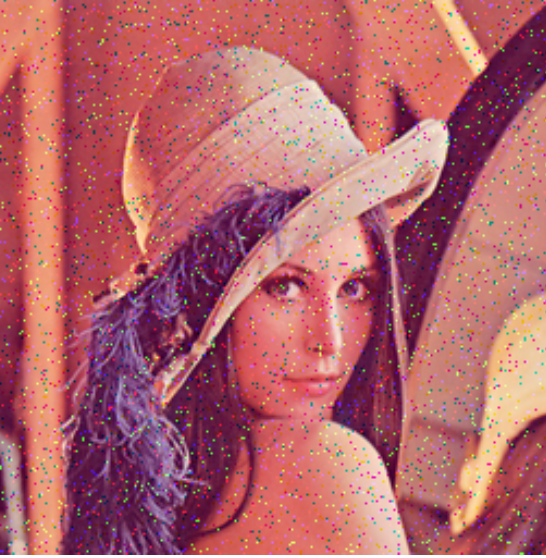
\includegraphics[width=0.9\linewidth]{images/result/figure6.png}
    \centering
    \end{subfigure}
    \caption{}
\end{figure}

Wang’s method has two parameters, $\mu$ and $\beta$, which are set as $\mu = 250$ and $\beta = 1$ by adjusting for this noise removal task through preliminary experiments. The proposed method with ‘Cross’ and ‘Square’ structuring elements shown in \textbf{Figure 2a} and \textbf{Figure 2b}, respectively.

\begin{figure}[H]
    \centering
    \begin{subfigure}[t]{.4\textwidth}
    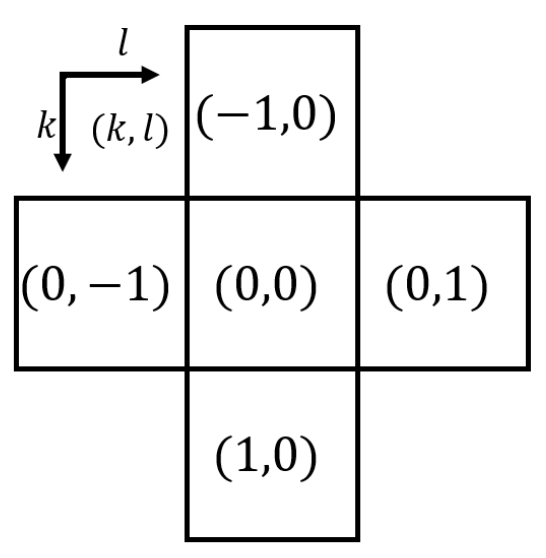
\includegraphics[width=0.9\linewidth]{images/result/cross.png}
    \centering
    \caption{}
    \end{subfigure}
    \begin{subfigure}[t]{.4\textwidth}
    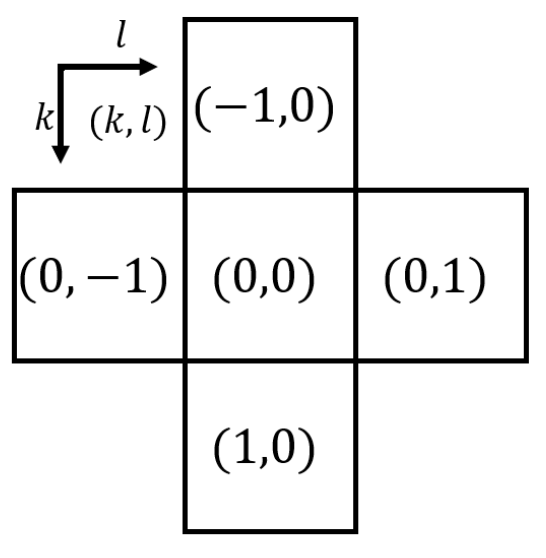
\includegraphics[width=0.9\linewidth]{images/result/square.png}
    \centering
    \caption{}
    \end{subfigure}
    \caption{}
\end{figure}

Below are the noise removal results using Wang’s method (\textbf{top} row) and the proposed order space-based morphological operations (\textbf{middle} and \textbf{bottom} rows) with $o^S$ for a noisy image in \textbf{Figure 1}, where their subcaptions denote the ‘operation/structuring element’ used for computing respective images: The top row shows the results of Wang’s method, where ‘HG’ indicates that the structuring elements are given by hypergraphs. The middle and bottom rows show the results of the proposed method with ‘Cross’ and ‘Square’ structuring elements shown in \textbf{Figure 2}. The six columns from left to right show the results of dilation (Dilat.), erosion (Eros.), opening (Open.), closing (Clos.), open–closing (O.-c.) and close–opening (C.-o.) operations, respectively.\\

\begin{figure}[H]
    \centering
    \begin{subfigure}[t]{.9\textwidth}
    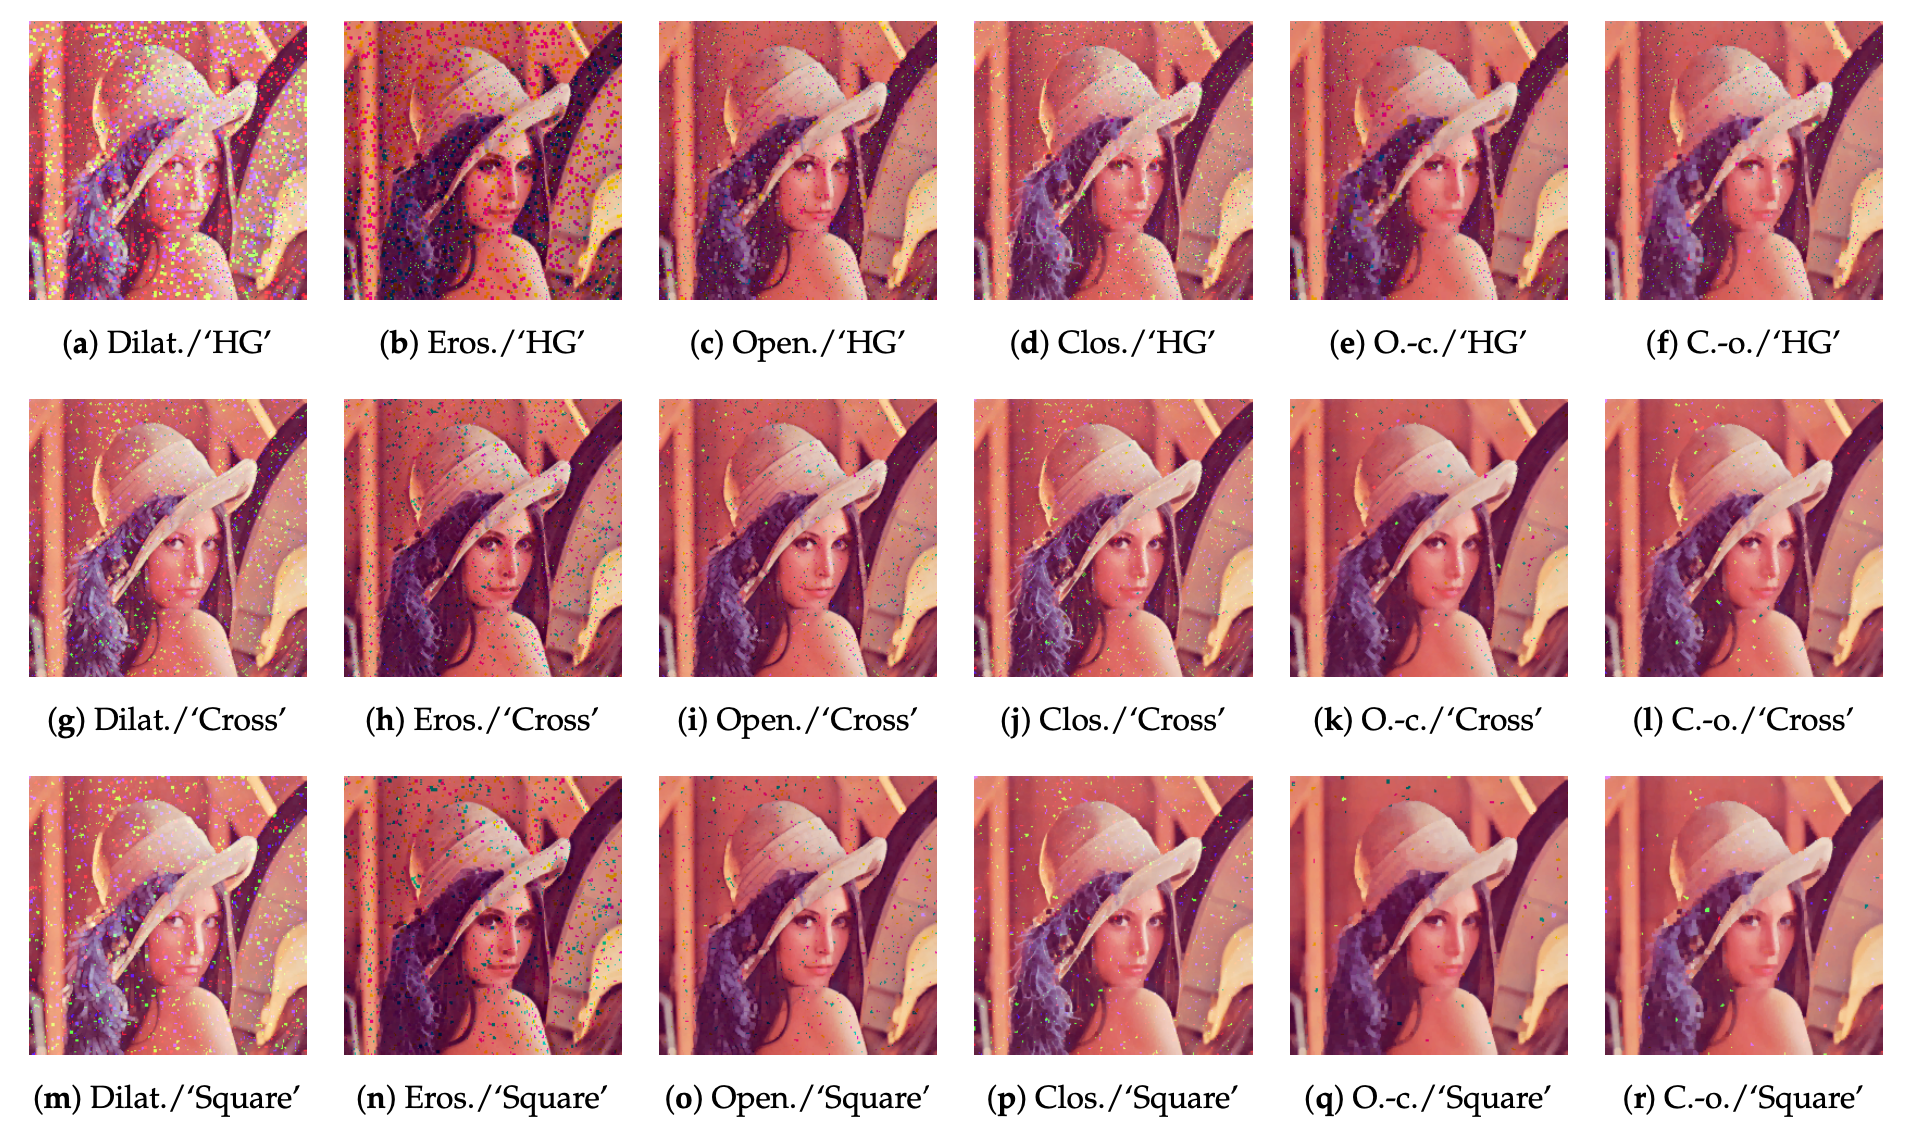
\includegraphics[width=0.9\linewidth]{images/result/result1.png}
    \centering
    \end{subfigure}
    \caption{}
\end{figure}


\textbf{Table 1} shows the values of the peak signal-to-noise ratio (PSNR) [25] between the output images in \textbf{Figure 1}

\begin{table}[H]
\caption{PSNR for output images in \textbf{Figure 1}}
\label{tab:psnr-tab}
\begin{tabular}{|l|l|l|l|l|l|l|}
\hline
SE       & Dilation & Erosion & Opening & Closing & Open-Closing & Close-Opening \\ \hline
'HG'     & 15.31    & 16.22   & 20.11   & 20.52   & 20.88        & 21.59         \\ \hline
'Cross'  & 18.82    & 18.80   & 22.96   & 23.11   & 25.14        & 25.13         \\ \hline
'Square' & 17.79    & 17.73   & 23.67   & 23.97   & 25.74        & 25.83         \\ \hline
\end{tabular}
\end{table}

The performance of noise removal is evaluated by the mean PSNR among the 12 different images as summarized in \textbf{Figure 4}, where \textbf{Figure 4a, 4b} show the results of open–closing and close–opening, respectively. In each graph, the vertical and horizontal axes denote the mean PSNR among the 12 images and the density of impulse noise varying from $10\%$ to $60\%$, respectively, and the line colors, blue, orange, green and red correspond to Wang’s method and the proposed methods with $o^S$, $o^P$ and $o^M$, respectively. In both graphs, Wang’s method (blue line) obtains higher values of mean PSNR than the proposed methods with $o^P$ and $o^M$ (green and red lines), and the proposed method with $o^S$ (orange line) outperforms Wang’s method.

\begin{figure}[H]
    \centering
    \begin{subfigure}[t]{.4\textwidth}
    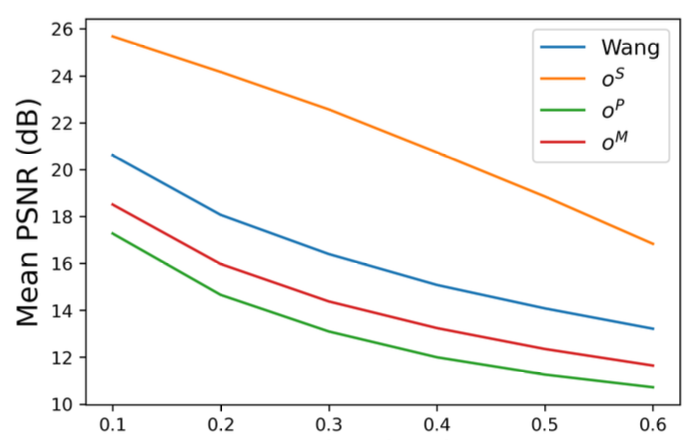
\includegraphics[width=0.9\linewidth]{images/result/open-closing.png}
    \centering
    \caption{Open-Closing}
    \end{subfigure}
    \begin{subfigure}[t]{.4\textwidth}
    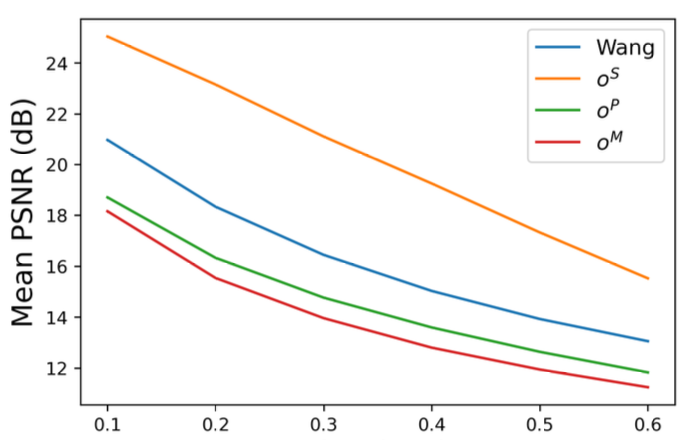
\includegraphics[width=0.9\linewidth]{images/result/close-opening.png}
    \centering
    \caption{Close-Opening}
    \end{subfigure}
    \caption{}
\end{figure}


They also compared the performance of grayscale and color morphological operations as illustrated in \textbf{Figure 5}, where a color original image (top left box) is corrupted by Gaussian or impulse noise to produce a noisy image (top right box).

\begin{figure}[H]
    \centering
    \begin{subfigure}[t]{.9\textwidth}
    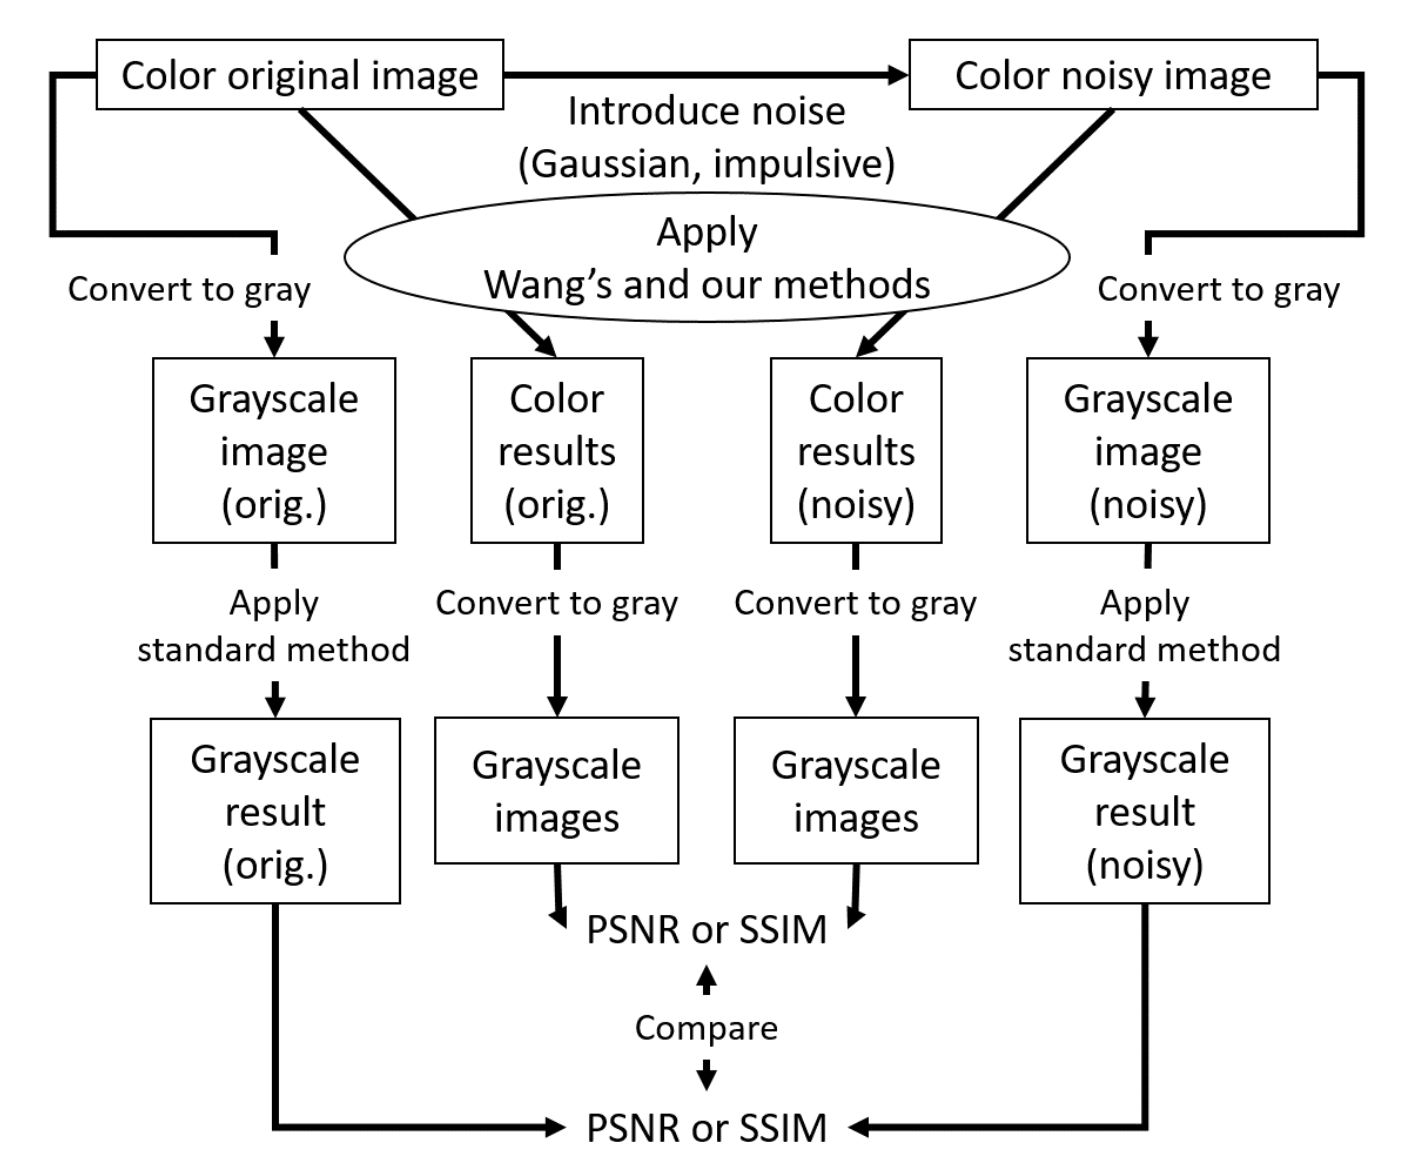
\includegraphics[width=0.9\linewidth]{images/result/flow.png}
    \centering
    \end{subfigure}
    \caption{}
\end{figure}

\textbf{Figure 6} shows the results of \textbf{Gaussian noise} removal with the SIDBA dataset, where the vertical axes denote \textbf{Figure 6a} PSNR and\textbf{ Figure 6b} SSIM, and the horizontal axes denote the compared methods. In this figure, the grayscale operation achieved the highest PSNR and SSIM values, and the proposed method outperformed Wang’s method.

\begin{figure}[H]
    \centering
    \begin{subfigure}[t]{.4\textwidth}
    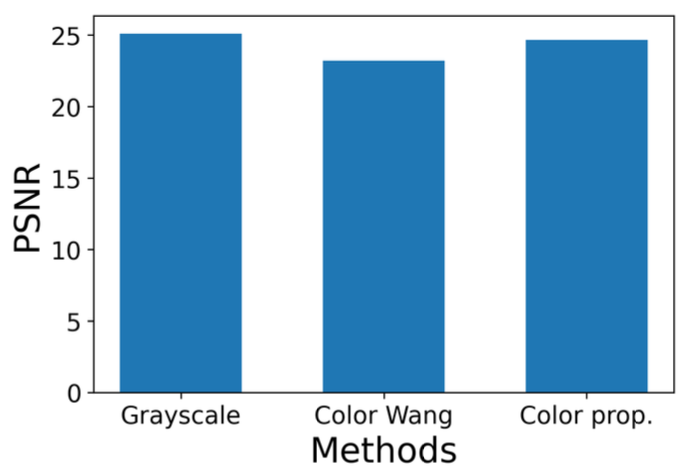
\includegraphics[width=0.9\linewidth]{images/result/PSNR_gaussian.png}
    \centering
    \caption{PSNR vs.methods}
    \end{subfigure}
    \begin{subfigure}[t]{.4\textwidth}
    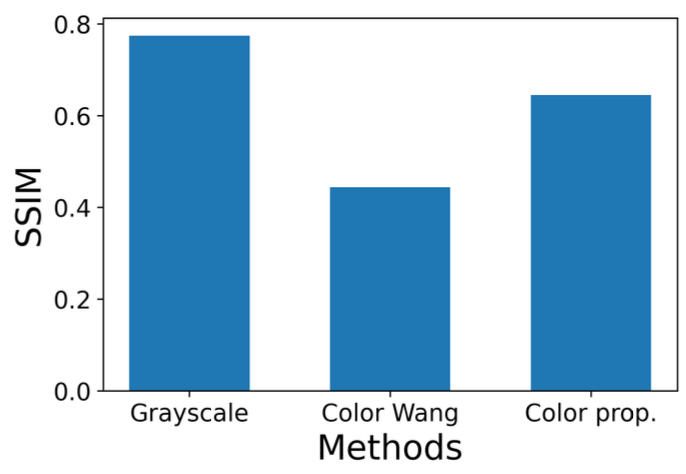
\includegraphics[width=0.9\linewidth]{images/result/SSIM_gaussian.png}
    \centering
    \caption{SSIM vs. methods}
    \end{subfigure}
    \caption{Results of Gaussian noise removal}
\end{figure}

\textbf{Figure 7} shows the results of impulse noise removal, where the settings of axes are the same as \textbf{Figure 6}. In \textbf{Figure 7a}, the proposed method achieved the highest PSNR value, while in \textbf{Figure 7b}, the grayscale operation achieved the highest SSIM value. The reason why the grayscale operation achieves higher values than color ones is speculated to be that the conversion from color to gray has a noise-reduction effect.

\begin{figure}[H]
    \centering
    \begin{subfigure}[t]{.4\textwidth}
    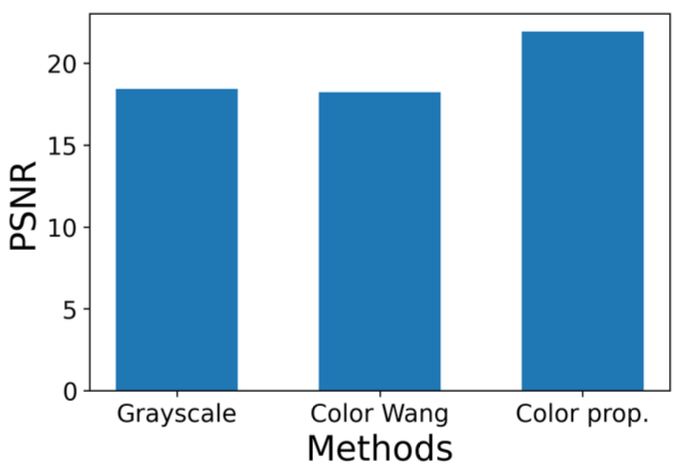
\includegraphics[width=0.9\linewidth]{images/result/PSNR_impulse.png}
    \centering
    \caption{PSNR vs.methods}
    \end{subfigure}
    \begin{subfigure}[t]{.4\textwidth}
    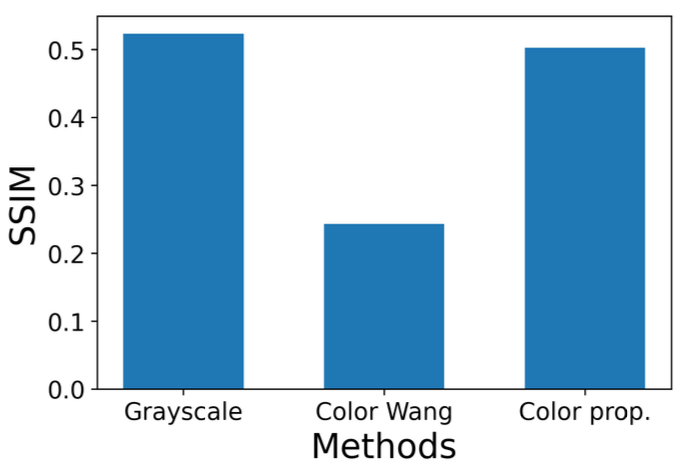
\includegraphics[width=0.9\linewidth]{images/result/SSIM_impulse.png}
    \centering
    \caption{SSIM vs. methods}
    \end{subfigure}
    \caption{Results of impulse noise removal}
\end{figure}

The above speculation is investigated in \textbf{Table 2}, where color noisy images are compared with grayscale noisy images by PSNR and SSIM for Gaussian and impulse noises. The values of the image quality measure for R, G and B components are improved by grayscale conversion for all combinations of noises and measures. This result shows that the grayscale conversion has a noise-reduction effect. In terms of the color morphological operations in this experiment, the proposed method achieved better PSNR and SSIM values than Wang’s method.

\begin{table}[H]
\centering
\caption{Comparison of the quality of noisy images between color and gray}
\label{tab:comp-tab}
\begin{tabular}{|llllll|}
\hline
Noise    & Quality Measure & R     & G     & B     & Gray           \\ \hline
Gaussian & PSNR            & 18.90 & 19.06 & 19.03 & \textbf{22.71} \\
Gaussian & SSIM            & 0.306 & 0.350 & 0.315 & \textbf{0.417} \\
Impulse  & PSNR            & 12.16 & 11.94 & 12.01 & \textbf{16.63} \\
Impulse  & SSIM            & 0.118 & 0.144 & 0.122 & \textbf{0.183} \\ \hline
\end{tabular}
\end{table}

Next, they show the experimental results for the fuzzy morphological operations. \textbf{Figure 8} shows the PSNR values for different values of $\alpha$ varying from $0.1$ to $1.0$, where we applied the fuzzy open–closing to the noisy image in \textbf{Figure 1}. We observe that $\alpha = 0.5$  achieves the highest PSNR value, and use $\alpha = 0.5$ below.

\begin{figure}[H]
    \centering
    \begin{subfigure}[t]{.6\textwidth}
    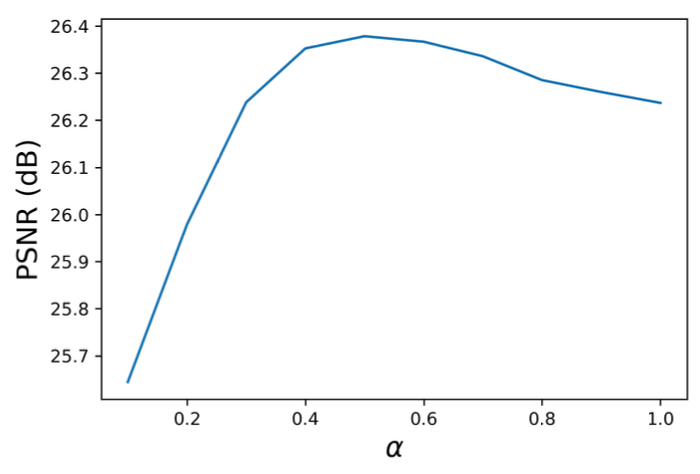
\includegraphics[width=0.9\linewidth]{images/result/alpha.png}
    \centering
    \end{subfigure}
    \caption{}
\end{figure}

\textbf{Figure 9} shows the results of the proposed fuzzy morphological operations. The order of the output images (a–f) by six morphological operations, dilation (Dilat.), erosion (Eros.), opening (Open.), closing (Clos.), open–closing (O.-c.) and close–opening (C.-o.).

\begin{figure}[H]
    \centering
    \begin{subfigure}[t]{.9\textwidth}
    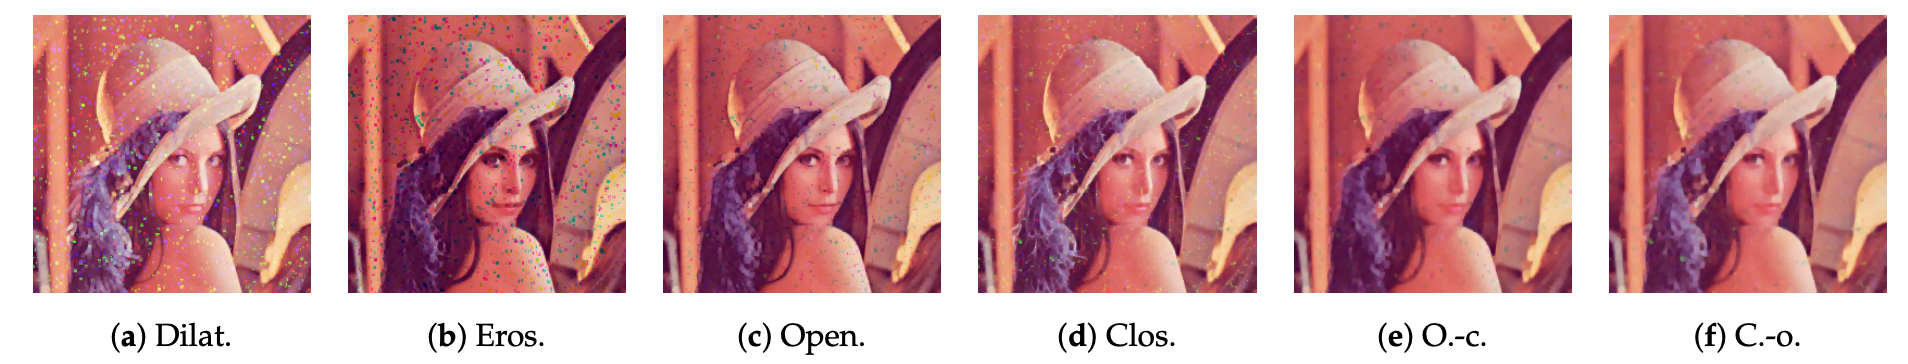
\includegraphics[width=0.9\linewidth]{images/result/fuzzy.png}
    \centering
    \end{subfigure}
    \caption{}
\end{figure}

\textbf{Figure 10} shows the effectiveness quantitatively by comparing the mean PSNR values computed with the SIDBA dataset between crisp and fuzzy operations, where the vertical and horizontal axes denote the mean PSNR and noise density as well as the settings from \textbf{Figure 4}, and \textbf{Figure 10a,b} which show the results of open–closing and close–opening operations, respectively. For both operations, the fuzzy ones denoted by purple lines outperform the crisp ones denoted by orange lines.

\begin{figure}[H]
    \centering
    \begin{subfigure}[t]{.9\textwidth}
    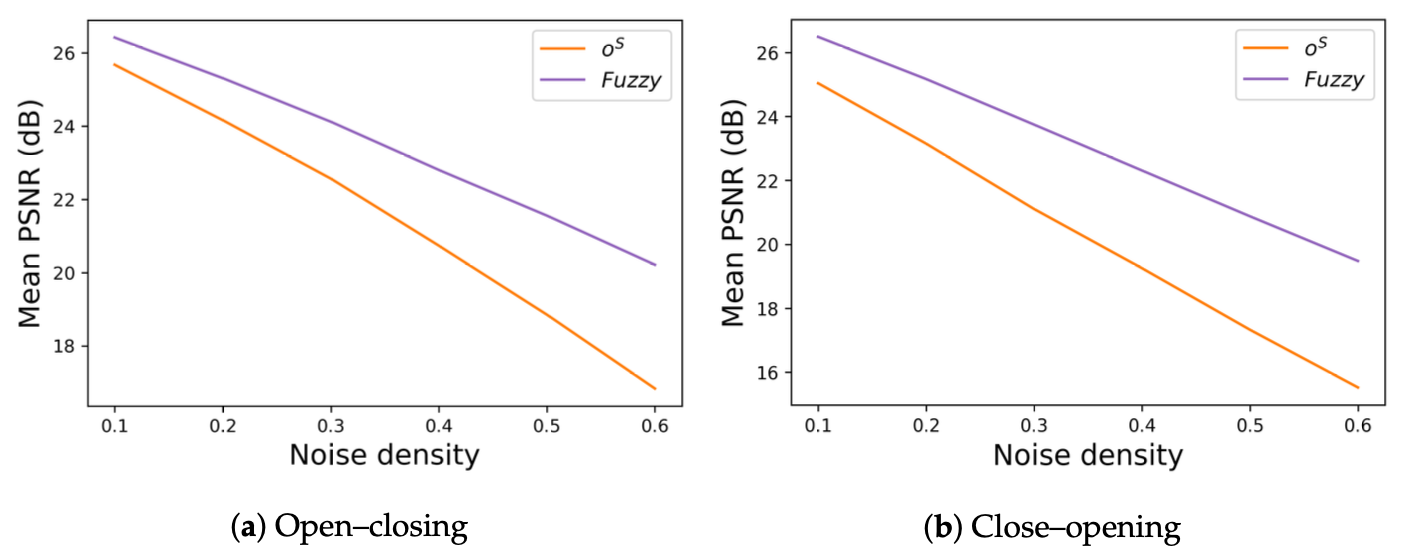
\includegraphics[width=0.9\linewidth]{images/result/crisp_vs_fuzzy.png}
    \centering
    \end{subfigure}
    \caption{}
\end{figure}

% \newpage

\section*{Discussion and Conclusion}

\begin{itemize}
    \item The proposed method is a method by which the obtained three orders, which form a 3D order space, can be unified into a single order of pixels in a suitable manner for a given application.
    \item The ways of unifying three orders are not restricted to the three methods presented in this paper. Investigating better ways to unify plural orders into one will be a promising future research direction.
    \item Extended the proposed order space-based morphological operations to their fuzzy version, where we proposed a method for fuzzifying morphological operations by exponentially weighted averaging.
    \item The noise removal performance was further improved by the fuzzification for both open–closing and close–opening op- erations, both of which achieved better performance than dilation, erosion, opening and closing operations in a conventional crisp situation.
    \item Future work will includethe extension of the proposed method for color image processing to multidimensional data processing, which will also be fuzzified by the proposed exponentially weighted averaging method to improve the performance.
\end{itemize}